\documentclass[11pt, a4paper]{article}
\usepackage{graphicx} % inserting pictures
\usepackage[dvipsnames]{xcolor} % additional colours
\usepackage{minted} % python typesetting
\usemintedstyle{vs} 
\usepackage{xcolor} % accessing the named colour LightGray
\usepackage{hyperref} % hyperlinks for contents
\usepackage{setspace} % customising line spacing
\usepackage{ragged2e} % RaggedRight
\usepackage{fancyhdr} % Headers and footers
\usepackage[utf8]{inputenc} 
\DeclareUnicodeCharacter{2609}{\circle}

\hypersetup{
colorlinks=true,
citecolor=black
} % making the links colored

\definecolor{LightGray}{gray}{0.9} % background colour for python code

\renewcommand{\thefootnote}{\textcolor{black}{\arabic{footnote}}}
\let\footnote=\endnote

\pagestyle{fancy}
\fancyhead{}
\fancyhead[L]{\slshape\nouppercase{\leftmark}}

\fancyfoot{}
\fancyfoot[C]{\thepage}

\begin{document}

% Title Page

\doublespacing{\title{\Huge {\vspace{2.5cm}} \textbf{Modelling the 
Climate and Energy Balance of an Earth-Like Planet} \\ {\vspace{20mm}}
\huge Computational Physics Prize 2023 \\ {\vspace{0.25cm}}}}
\author{\LARGE Eric Ayivor KS \\}

\maketitle
\begin{center}
\vspace{3cm}
\LARGE \textbf{Eton College}
\end{center}

\thispagestyle{empty}

% Contents Page
\newpage
{
  \singlespacing{
  \hypersetup{linkcolor=BrickRed}
  \tableofcontents
  }
}

% Introduction
\newpage
\section{Introduction\label{introduction}}
\onehalfspacing{This project aims to numerically model the climate of an 
earth-like planet by predicting its temperature over time and investigate 
how changing factors such as distance from the star and emissivity of the 
planet's atmosphere can have a profound impact on the climate.}

\subsection{Dependencies and distribution\label{dependencies-and-distribution}}
\onehalfspacing{The dependencies used in this project are NumPy and 
MatPlotLib's Pyplot function. Specifically from NumPy, the constant $\pi$ 
is imported directly.}

\subsubsection{Files\label{files}}
\onehalfspacing{\begin{itemize} \item climate\_modelling.py is the 
complete model with a few functions for plotting and analysis. This is 
all explained in section 4 - Usage \item climate\_modelling.pdf is this 
document, including the code, graphs and this project \item 
climate\_modelling.tex is the LaTeX code required to build \\
climate\_modelling.pdf \end{itemize}}

\subsubsection{Experimenting\label{experimenting}}
\onehalfspacing{To experiment, you can either import the classes and model 
function into a new python file to preserve the original model, or you can 
simply edit the parameters in the original file, such as change LUMINOSITY 
to 2*LUMINOSITY, which would probably be easier.}

\subsection{Background: Climate Modelling}
\onehalfspacing{Climate modelling is the process of using computer 
simulations to predict how the Earth's climate will change over time. This 
field of study is a relatively new one, having begun in the 1960s, and has 
since evolved to become an essential tool for scientists and amateurs like 
myself to understand the complex processes that shape our planet's climate. \\}

\onehalfspacing{\noindent{Climate models work by incorporating various 
factors that affect the Earth's climate, such as greenhouse gas emissions, 
solar radiation, and ocean currents. By inputting data on these factors, 
scientists can create models that predict how the Earth's climate will 
change over time. These models are tested against historical data to verify 
their accuracy and are continually updated as new information becomes 
available. \\}}

\onehalfspacing{\noindent{My model is rather more simplistic, taking into 
account the same broad factors and processes, but simplifying them into a 
way that my GCSE Maths and Science understanding could cope with. I had to 
do a fair bit of research to compensate for my lack of knowledge, but 
because all the prior similar work is far more complex and rigorous than I 
could hope to deal with, much of what follows is my own work and deductions 
in order to create a model that is atleast semi-accurate and simple enough 
for me to understand everything that is going on. There was no point making 
a model too complex for me to understand by modifying prior work as it 
negates the point of the project, which for me, was to try and gain a deeper 
understanding of the processses that affect our planet and it's climate. \\}}

\onehalfspacing{\noindent{Overall, climate modelling is a vital tool in our 
efforts to understand and mitigate the impacts of climate change, and its 
continued development is critical to our ability to address this global 
challenge. \\}}

\onehalfspacing{\noindent{At first I tried to make a model that was atleast 
95\% accurate to current global temperatures, but I had neither the time nor 
the knowledge to make that work, so I decided to attempt to create one that 
was atlest 60\% accurate. I achieved this goal as my final model was around 
75\% accurate, that too only considering the first 1000 years of an early 
Earth. I am confident that it would become more accurate given the time for 
billions of iterations to match the billions of years that our Earth has 
been around. \\}}

\subsection{Summary of Results}
\onehalfspacing{My results gave an average global temperature of around 
200K, and average temperature of around 180K for high latitudes and around 
230K for equatorial ones. }

% Mathematical Details
\newpage
\section{Mathematical Details\label{mathematical-details}}

% Energy Input (Global and Local)
\subsection{Calculating Energy Input\label{calculate-energy-input}}
\subsubsection{Intensity of global solar insolation \label{global-solar-
insolation}}

\onehalfspacing{The first and easiest step was calculating the energy 
input from the sun for each latitude band. The most commonly used value 
for the intensity of solar intensity is approximately 1400 Wm$^{-2}$.
In my first attempts at making this model, I simply used this value
as a constant, however creating a function to calculate the energy
input makes it easier to experiment later, for example by varying
the distance of the planet in AU. The light intensity that reaches
the top of the planet’s atmosphere from the sun is given by the
following equation:}

\doublespacing{\[I = \frac{L}{4\pi D^{2}}\]}

\onehalfspacing{\noindent where L is the luminosity of the star and 
D is its distance from the planet. These values are initialised to 
1L and 1AU by default to match the Earth’s parameters but they can 
be easily modified to experiment with their effect on the planet’s
climate. For the purposes of the model, we divide this value by 4
because the circular area that is actually exposed to solar
radiation at any one time ($\pi r^2$) is 4 times smaller than the
surface area of the planet that could be exposed to solar radiation
($4\pi r^2$). This gives us the value of approximately 1361
Wm$^{-2}$ in total, and approximately 340 Wm$^{-2}$ reaching the
surface.}

\subsubsection{Intensity of local solar insolation\label{local-solar-
insolation}}

\onehalfspacing{The exact light intensity that reaches the Earth’s surface 
is dependent on 2 additional factors: latitude, and albedo. Because 
the earth’s surface is spherical, the energy reaching the polar 
latitudes is spread out over a larger surface area, reducing the 
intensity. Furthermore, the earth is not a perfect blackbody so the 
albedo means that a proportion of the received radiation will be 
reflected. This leads to the following equation:}

\doublespacing{\[j=I cos{\theta} A\]}

\onehalfspacing{\noindent where j is the light intensity in Wm$^{-2}$ at 
each latitude, $\theta$ is the average angle of the latitude band 
(for example between 85 and 90 degrees, $\theta=87.5$), and A is 
the albedo of the latitude band. Albedo is calculated based on the 
composition of the latitude band in terms of water, ice / snow, and 
dry land. At the start of the model, every latitude band is 
initialised in the same way reflecting the approximate composition 
of the earth. Every latitude band starts off as 71\% water, 12\% 
permanent ice and 19\% dry land, approximately in line with the 
average composition of the planet \cite{1}. As time 
progresses and the model evolves, the composition changes. For example, the 
model assumes that every latitude with a temperature below -10$^{\circ}$ C 
(263K) is snow covered, thus affecting the albedo for the next 
iteration of the model.}

\subsection{Calculating Meridional Heat Transport\label{calculate-
meridional-heat-transport}} 
\onehalfspacing{Probably the most challenging part of the model was 
calculating the heat transport to and from neighbouring latitude bands, 
known as meridional heat flow. In order to calculate this, we have to use 
the concepts of heat flux and heat flux density. \\}

\onehalfspacing{\noindent{Heat flux ($\phi$) is defined as the rate of 
heat energy transfer through a given service (W) and heat flux density 
($\phi_q$) is heat flux per unit area (Wm$^{-2}$ \cite{2}). We are trying 
to calculate heat flux density, which is given by the following equation
\cite{3}:}}

\doublespacing{\[\phi_q=-k\nabla t\]}

\onehalfspacing{\noindent{where the negative sign denotes that heat always 
travels from higher to lower temperature zones, $k$ is the thermal 
conductivity of the material (in this case the ocean or the atmosphere) in 
Wm$^{-1}$K$^{-1}$ and $\nabla t$ is the temperature gradient in Km$^{-1}$.}}

\doublespacing{\[\nabla t = \frac{\Delta t}{d}\]}

\onehalfspacing{\noindent{The change in temperature $t$ can be calculated 
using the Stefan-Boltzmann Law  using $j$ which was calculated in the 
previous section. Then, we consider the greenhouse effect to find $t$ for 
each latitude band before meridional heat transport. The Stefan-Boltzmann 
Law \cite{4} is as follows:}}

\doublespacing{\[j = \sigma T^4\]}

\onehalfspacing{\noindent{Rearranging for surface temperature in kelvin 
gives:}}

\doublespacing{\[T_{surface} = \sqrt[4]{\frac{j}{\sigma}}\]}

\onehalfspacing{\noindent{This temperature is much colder than expected, 
however, due to the lack of consideration for the greenhouse effect. The 
effects of the greenhouse effect can be summarised in the following equation 
\cite{5}: }}

\doublespacing{\[T_{greenhouse}=T_{surface}\left[\frac{1}{1-\frac{\epsilon}
{2}}\right]^\frac{1}{4}\] \[T_{greenhouse}=\sqrt[4]{\frac{j}
{\sigma}}\times\left[\frac{1}{1-\frac{\epsilon}{2}}\right]^\frac{1}{4}\]}

\onehalfspacing{\noindent{Therefore $\Delta$ t is as follows: }}

\doublespacing{\[\Delta t=T_{greenhouse_1}-T_{greenhouse_2}\]}

\onehalfspacing{\noindent{The distance d between any two latitude bands can 
be approximated as the distance along the Earth’s surface between the 
midpoint angle of the two latitude bands. For example, between the latitude 
bands (85$^{\circ}$ - 90$^{\circ}$) and (80${^\circ}$ - 85${^\circ}$), $d$ 
can be approximated as the distance along the Earth’s surface between the 
latitude line at 87.5$^{\circ}$N and the latitude line at 82.5$^{\circ}$N. 
In the general case:}}

\doublespacing{\[d=r\times\Delta\theta\times cos(\theta)\]}

\onehalfspacing{\noindent{where r is the radius of the earth in m, and 
$\theta$ is the angle between the 2 latitude bands in radians, which for the 
purposes of this model will always be $\frac{5\pi}{180}$ because this model 
deals with discrete latitude bands in 5-degree increments. \\}}

\onehalfspacing{\noindent{Meridional heat flow is primarily composed of 
contributions from oceanic and atmospheric circulation (Enderton, 2009) 
\cite{6} in the approximate ratio of 3:7 (Wunsh, 2007) \cite{7}. Thus, we 
create two new constants representing the proportional contributions: 
$P_{\mathrm{AIR}}$ = 0.7 \& $\mathrm{P_{OCEAN}}$ = 0.3}}

\onehalfspacing{\noindent{Substituting accordingly gives:}}

\doublespacing{\[\phi_q=\frac{-k\Delta t}{r\times\Delta\theta\times 
cos(\theta)}\]}

\onehalfspacing{\noindent{Accounting for the relative contributions of the 
ocean and atmosphere and then factorising gives:}}

\doublespacing{\[\phi_q=\frac{\Delta t(P_{\mathrm{AIR}}\times -
k_{\mathrm{AIR}}+(P_{\mathrm{OCEAN}}\times -k_{\mathrm{OCEAN}})}
{r\times\Delta\theta\times cos(\theta)}\]}

\begin{center}
\onehalfspacing{where k$\mathrm{_{AIR}=0.025}$ and k$\mathrm{_{OCEAN}=0.592}$
\cite{8}}
\end{center}

\onehalfspacing{\noindent{which is the final equation form that I use to 
calculate meridional heat transport in Wm$^{-2}$.}}

\subsection{Updating latitude composition \label{latitude-composition}}
\onehalfspacing{After each year of the simulation, the albedo must be 
updated to reflect changes in temperature. The way I handled this was as 
follows: \\}

\onehalfspacing{\noindent{For every time increment, for every latitude band, 
if the average temperature of that latitude band is less than 263.15 K 
(-10$^\circ$ C), the percentage of ice will increase by a certain percentage 
and the percentage of water will decrease accordingly. This will continue 
until the percentage of water becomes too low, at which point the ice is set 
to 100\% and the ice band is 100\% iced over. \\}}

\onehalfspacing{\noindent{The only mathematical part of this process was 
determining by what percentage the ice should increase. I couldn’t find any 
suitable data in my research, so I decided to estimate an appropriate parameter. \\}}

\onehalfspacing{\noindent{I found that the Antarctic Ice Sheet contains 
about 26.5 million cubic kilometres of ice and is losing about 150 billion 
tons of ice per year. \\}}

\onehalfspacing{\noindent{The density of ice is 916.7 kg/m$^3$  and to 
convert between km$^3$ and m$^3$ you simply multiply by $10^9$. Density is 
mass divided by volume, so the mass of the Antarctic Ice Sheet is 
approximately $2.429\times{10}^{19}$ kg or $2.429\times{10}^{16}$ tons 
(which is 99.6\% accurate to the value on Wikipedia). This means that the 
Antarctic Ice Sheet is losing $6.175\times{10}^{-6}$\% every year. Given 
this is accelerated by human activities quite significantly and assuming 
that the ice sheet would gain ice at approximately the same rate that it 
loses ice, in my model, for every year that the temperature of the latitude 
band remains below 263.15 K, the percentage of ice increases by 
$5\times{10}^{-6}$\% and is therefore multiplied by 1.000005. The value of 
water decreases appropriately to accommodate this. \\}}

\subsubsection{Other details\label{other-details}}

\onehalfspacing{\noindent{On a similar but not entirely related note, the 
Earth's climactic processes do not remain exactly the same throughout it's 
orbit around the sun. Because the earth's orbit is very circular but still 
partially elliptical, variations in the Earth's orbit called Milkankovitch 
cycles must be considered. In total, Milkankovitch cycles can cause 
variations of up to 25\% of the insolation reaching the Earth's surface 
\cite{11}. Variations in eccentricity (how close to a circle Earth's orbit 
is) occur in cycles of around 100,000 years \cite{12} and variations in 
obliquity (the Earth's tilt) take place in cycles of around 41,000 years. 
\cite{13}. Also, every few thousand years, CO$_2$ levels naturally 
fluctuate, changing the emissivity of the atmosphere. Over the past several 
hundred thousand years, CO$_2$ and other greenhouse gas concentrations hjave 
been on average rising. Because this is a very simplistic model, I included 
all of these effects in a simple \textit{if} statement. Every 50,000 years, 
the emissivity increases by 2\%, the global insolation increases or 
decreases by 25\%, and obliquity changes apparently have no discernible 
effect on insolation \cite{14}. Given more time and a better understanding 
of the complexity of Earth's natural cycles and patterns I would love to 
more accurately implement these processes, but this will have to do for now.}

\newpage
\section{Overview of Model\label{overview-of-model}}
\onehalfspacing{My simulation uses a fixed time step assumed to be 1 year on 
Earth and can be summarised simply as follows:}

\onehalfspacing{\begin{enumerate}
\item Initialise a planet and it's relationship with its main star
\item Calculate the temperature after meridional heat transfer etc.
\item Repeat all steps as many times as required (time is initialised to 
500,000 365 day years
\end{enumerate}}

\subsection{Flow\label{flow}}
\subsubsection{Initialisation\label{initialisation}}
\onehalfspacing{At the start of the program, a class called Constants is 
created which is inherited by the main class of the model. This contains the 
constants which are initialised at the start of the model. The values in the 
constants class will never change and should ideally not be experimented 
with, though it is possible. These are:}

\begin{minted}
[
baselinestretch=1.2,
bgcolor=LightGray,
fontsize=\footnotesize,
linenos
]
{python}
STEFAN = 5.67e-8        # Stefan's Constant (Wm-2K-4)
ALBEDO_LAND = 0.2       # average albedo of dry land                  
ALBEDO_ICE = 0.85       # average albedo of ice / snow covered land
ALBEDO_WATER = 0.4      # average albedo of open water (oceans / seas)
K_AIR = 0.025           # thermal conductivity of air
K_OCEAN = 0.592         # thermal conductivity of (sea)water
\end{minted}

\subsection{Parameters}
\onehalfspacing{\noindent{The model takes in certain parameters which are used to set up the Planet class. These are luminosity of the star, distance 
from the star, radius of the planet emissivity of the atmosphere, and the 
relative contributions of air and ocean to meridional heat transport.}}

\begin{minted}
[
breaklines,
baselinestretch=1.2,
bgcolor=LightGray,
fontsize=\footnotesize,
linenos
]
{python}
LUMINOSITY = 3.828e26     # luminosity of the star (W) - initialised to 1 L
DISTANCE = 1495978707e2   # distance from planet to star (m) - initialised to 1 AU
RADIUS = 63781e2          # radius of the planet (m)
EMISSIVITY = 0.78         # radius of the planet (m)
P_AIR = 0.7               # atmospheric contribution to meridional heat    transport
P_OCEAN = 0.3             # oceanic contribution to meridional heat transport
YEARS = 500000            # length of simulation in years
\end{minted}

\subsection{Things not worth including}
\onehalfspacing{If you change the length of the time step in months (that 
is, if you make every year longer, there will be no discernible effect of 
results except that the temperatures of each latitude band will get closer 
due to more meridional heat transfer but there will be no other change in 
results. Therefore, even if you change the distance between the planet and 
the star, there is no point changing the length of the year.}

\newpage
\section{Usage\label{usage}}
\begin{minted}
[
breaklines,
baselinestretch=1.2,
bgcolor=LightGray,
fontsize=\footnotesize,
linenos
]
{python}
### Libraries
import numpy as np                   # NumpPy
from matplotlib import pyplot as plt # MatPlotLib
from numpy import pi                 # Pi

class Constants:
    STEFAN = 5.67e-8        # Stefan's Constant (Wm-2K-4)
    ALBEDO_LAND = 0.2       # average albedo of dry land                  
    ALBEDO_ICE = 0.85       # average albedo of ice / snow covered land
    ALBEDO_WATER = 0.4      # average albedo of open water (oceans / seas)
    K_AIR = 0.025           # thermal conductivity of air
    K_OCEAN = 0.592         # thermal conductivity of (sea)water

    def __init__(self) -> None:
        pass

class Planet(Constants):

    def __init__(self, luminosity: float, distance: float, radius: float, emissivity: float, pAIR: float, pOCEAN: float) -> None:
        super().__init__()
        self.luminosity = luminosity
        self.distance = distance
        self.radius = radius
        self.emissivity = emissivity
        self.P_AIR = pAIR
        self.P_OCEAN = pOCEAN

        self.global_intensity = (self.luminosity / (4 * pi * self.distance ** 2)) / 4

        self.latitudes = np.arange(87.5, -92.5, -5)

        self.composition = [[0.65, 0.19, 0.16] for i in range(int(len(self.latitudes)/3))]
        self.composition.extend([[0.81, 0.0, 0.19] for i in range(int(len(self.latitudes)/3))])
        self.composition.extend([[0.65, 0.19, 0.16] for i in range(int(len(self.latitudes)/3))])

        self.albedos = [(i[0] * self.ALBEDO_WATER + i[1] * self.ALBEDO_ICE + i[2] * self.ALBEDO_LAND) for i in self.composition]
        self.distances = [(self.radius * 5 * pi / 180 * np.cos(np.radians(theta * pi / 180)))/1000 for theta in self.latitudes]

    def local_intensity(self):
        latitudes = list(self.latitudes)
        local_intensity_array = [(self.global_intensity * np.cos(np.radians(theta)) * self.albedos[latitudes.index(theta)]) for theta in latitudes]

        return np.array(local_intensity_array)
    
    def surface_temperatures(self, intensity_array: list):
        surface_temperatures_array = [((j / self.STEFAN) ** 0.25) for j in intensity_array]
        
        return np.array(surface_temperatures_array)
    
    def delta_temperatures(self, temperatures_array: list):
        temperatures_array = list(temperatures_array)
        delta_temps = []
        one_to_eighteen = []
        nineteen_to_thirty_five = []

        for i in range(1, 19):
            delta_t = temperatures_array[i] - temperatures_array[i-1]
            one_to_eighteen.append(delta_t)

        for i in range(18, 36):
            delta_t = temperatures_array[i-1] - temperatures_array[i]
            nineteen_to_thirty_five.append(delta_t)
        
        delta_temps.append(one_to_eighteen)
        delta_temps.append(nineteen_to_thirty_five)

        return np.array(delta_temps)

    def meridional_heat_transport(self, delta_temperatures_array: list):
        delta_temperatures_array = list(delta_temperatures_array)
        meridional_heat_transport = []
        lst1 = []
        lst2 = []

        for t in delta_temperatures_array[0]:
            distance = self.distances[list(delta_temperatures_array[0]).index(t)]
            phi = (t * ((self.P_AIR * -1 * self.K_AIR) + (self.P_OCEAN * -1 * self.K_OCEAN)))/distance
            lst1.append(phi)

        for t in delta_temperatures_array[1]:
            distance = self.distances[list(delta_temperatures_array[1]).index(t)]
            phi = (t * ((self.P_AIR * -1 * self.K_AIR) + (self.P_OCEAN * -1 * self.K_OCEAN)))/distance
            lst2.append(phi)

        meridional_heat_transport.extend(lst1)
        meridional_heat_transport.extend(lst2)

        return np.array(meridional_heat_transport)
    
    def greenhouse_temperatures(self, temperatures_array: list):
        greenhouse_temperatures = [temp * ((1 / (1 - self.emissivity / 2)) ** 0.25) for temp in temperatures_array]
        
        return np.array(greenhouse_temperatures)
    
    def update_intensity(self, input_array: list, meridional_transfer_array: list):
        input_array = list(input_array)
        for i in range(len(input_array) - 1):
            if i == 1:
                input_array[i] -= meridional_transfer_array[i]
            elif i <= int(len(input_array) / 2):
                input_array[i] += meridional_transfer_array[i-1]
                input_array[i] -= meridional_transfer_array[i]
            elif i > int(len(input_array) / 2) and i < len(input_array):
                input_array[i] += meridional_transfer_array[i+1]
                input_array[i] -= meridional_transfer_array[i] 
            elif i == len(input_array):
                input_array[i] -= meridional_transfer_array[i] 

        return input_array

    def update_albedos(self, latitude_temperatures_dictionary: dict):
        ice_list = []
        for latitude in latitude_temperatures_dictionary:
            if latitude_temperatures_dictionary[latitude][-1] > 263.15:
                ice = False
            else:
                ice = True
            ice_list.append(ice)
        for i in self.composition:
            if not ice_list[self.composition.index(i)]:
                i[0] = 0.81
                i[1] = 0.0
            else:
                update = i[1] * 0.00005
                if latitude_temperatures_dictionary[latitude][-1] > latitude_temperatures_dictionary[latitude][-2]:
                    i[0] += update
                    i[1] -= update
                else:
                    i[0] -= update
                    i[1] += update

def plot_latitude_temp(time: list, latitude_temps: dict, latitude):
    plt.plot(time, latitude_temps[latitude])
    plt.xlabel("Time / years")
    plt.ylabel("Temperature / degrees K")
    plt.grid(True)
    plt.show() 

def plot_global_temp(time: list, average_temps: np.ndarray):
    plt.plot(time, average_temps)
    plt.xlabel("Time / years")
    plt.ylabel("Temperature / degrees K")
    plt.grid(True)
    plt.show()

def model():
    LUMINOSITY = 3.828e26       # luminosity of the star (W) - initialised to 1 L
    DISTANCE = 1495978707e2     # distance from planet to star (m) - initialised to 1 AU
    RADIUS = 63781e2            # radius of the planet (m)
    EMISSIVITY = 0.78           # radius of the planet (m)
    P_AIR = 0.7                 # atmospheric contribution to meridional heat transport
    P_OCEAN = 0.3               # oceanic contribution to meridional heat transport
    YEARS = 1000                # length of simulation in years

    earth = Planet(luminosity=LUMINOSITY,
                   distance=DISTANCE,
                   radius=RADIUS,
                   emissivity=EMISSIVITY,
                   pAIR=P_AIR,
                   pOCEAN=P_OCEAN)
    
    average_temps_array = []
    latitude_temps_dictionary = {i:[] for i in (np.arange(87.5, -92.5, -5))}

    local_insolation_array = earth.local_intensity()

    year = 0

    while year < YEARS:
        surface_temps_array = earth.surface_temperatures(intensity_array=local_insolation_
        array)
        greenhouse_temps_array = earth.surface_temperatures(intensity_array=local_insolation_
        array)
            
        average_temps_array.append(np.mean(greenhouse_temps_array))
            
        for i in earth.latitudes:
            latitude_temps_dictionary[i].append(greenhouse_temps_array
            [list(earth.latitudes).index(i)])

        for i in range(12):
            delta_temps_array = earth.delta_temperatures(temperatures_array=greenhouse_
            temps_array)

            meridional_heat_transport_array = earth.meridional_heat_transport(delta_temperatures_array
            =delta_temps_array)

            local_insolation_array = earth.update_intensity(input_array=local_insolation_array,
            meridional_transfer_array=meridional_heat_transport_array)
                
        surface_temps_array = earth.surface_temperatures(intensity_array=local_insolation_
        array)
        greenhouse_temps_array = earth.greenhouse_temperatures(temperatures_array=surface_temps_
        array)

        for i in earth.latitudes:
            latitude_temps_dictionary[i].append(greenhouse_temps_array
            [list(earth.latitudes).index(i)])
            
        earth.update_albedos(latitude_temperatures_dictionary=latitude_
        temps_dictionary)

        change_intensity = 0.25 * earth.global_intensity

        if year % 50 == 0 and (year / 50) % 2 == 1:
            earth.emissivity *= 0.02
            earth.global_intensity += change_intensity
        elif year % 50 == 0 and (year / 50) % 2 == 0:
            earth.emissivity *= 0.02
            earth.global_intensity += change_intensity

        year += 1
    
    return np.array(average_temps_array), latitude_temps_dictionary

plot_global_temp(time=range(1000),
                 average_temps=model()[0])

plot_latitude_temp(time=range(2000),
                   latitude_temps=model()[1],
                   latitude=42.5)                   
\end{minted}

\newpage
\section{Data Analysis\label{data-analysis}}

\begin{center}
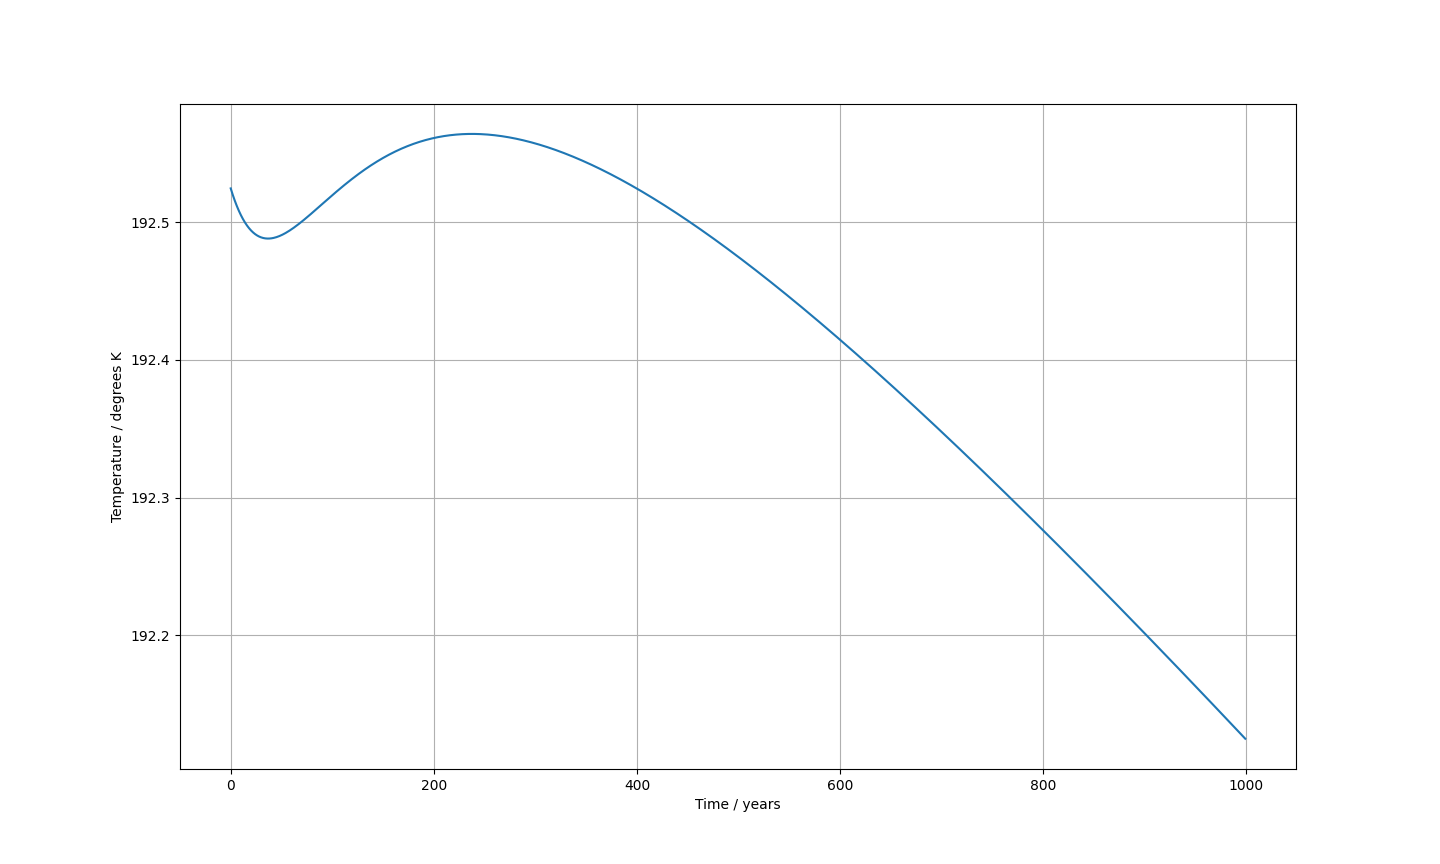
\includegraphics[scale=0.35]{Figure_1.png}
Global Average Temperature
\end{center}

\begin{center}
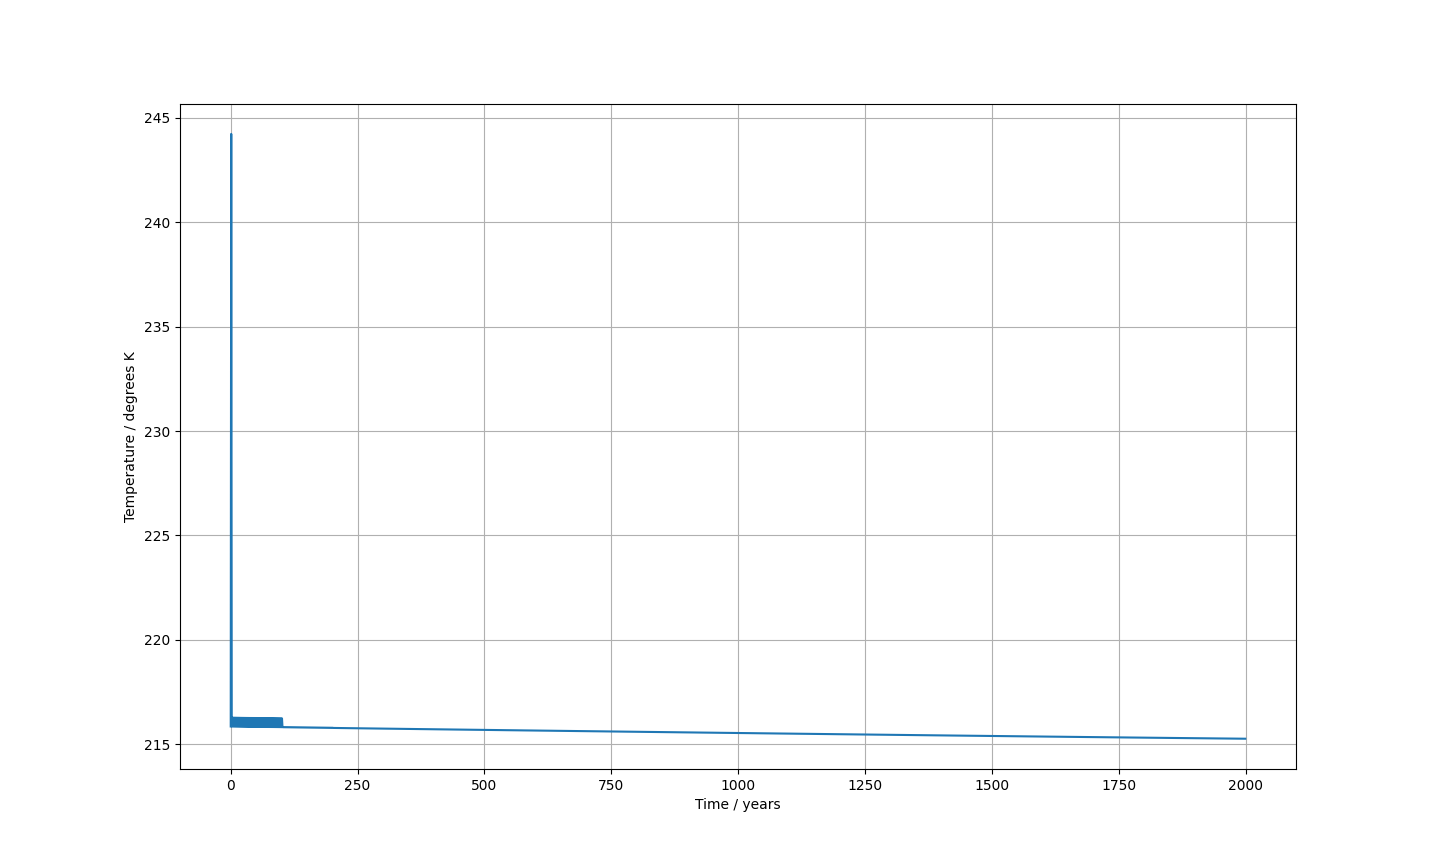
\includegraphics[scale=0.35]{Figure_2.png}
Average Temperature of 2.5 degrees North latitude band
\end{center}

\onehalfspacing{\noindent{Clearly the results produced by the model aren't 
wildly implausible but they are definitely not accurate to the current 
planet. The temperature seems to be consistently decreasing with occasional 
spikes despite the increeases in insolation caused by variations in 
eccentricity. I would like to think that 1 or 2 thousnad years is simply too 
small a timescale, and given longer to run (which I unfortunately don't have 
enough time for), the temperatures such correct themselves and eventually 
arrive at around 280 - 290K, which is the current average temperature. \\}}

\onehalfspacing{\noindent{However, it could also be that this model is 
simply too simplistic and lacks enough detail to make it viable. The results 
are correct to the nearest order of magnitude (which is a large jump from 
200K to 280K in terms of life-sustaining temperatures), but perhaps there 
have simply been too many shortcuts and assumptions taken regarding the 
maths and modelling. \\}}

\onehalfspacing{\noindent{The data is around 70 - 75\% accurate. In terms of 
machine learning, that would be considered a great model \cite{15}, however 
I think that even working within the constraints of this prize, the model 
could be improved a lot to make its accuracy more reliable. A longer runtime 
capacity would significantly aid this.}

\begin{center}
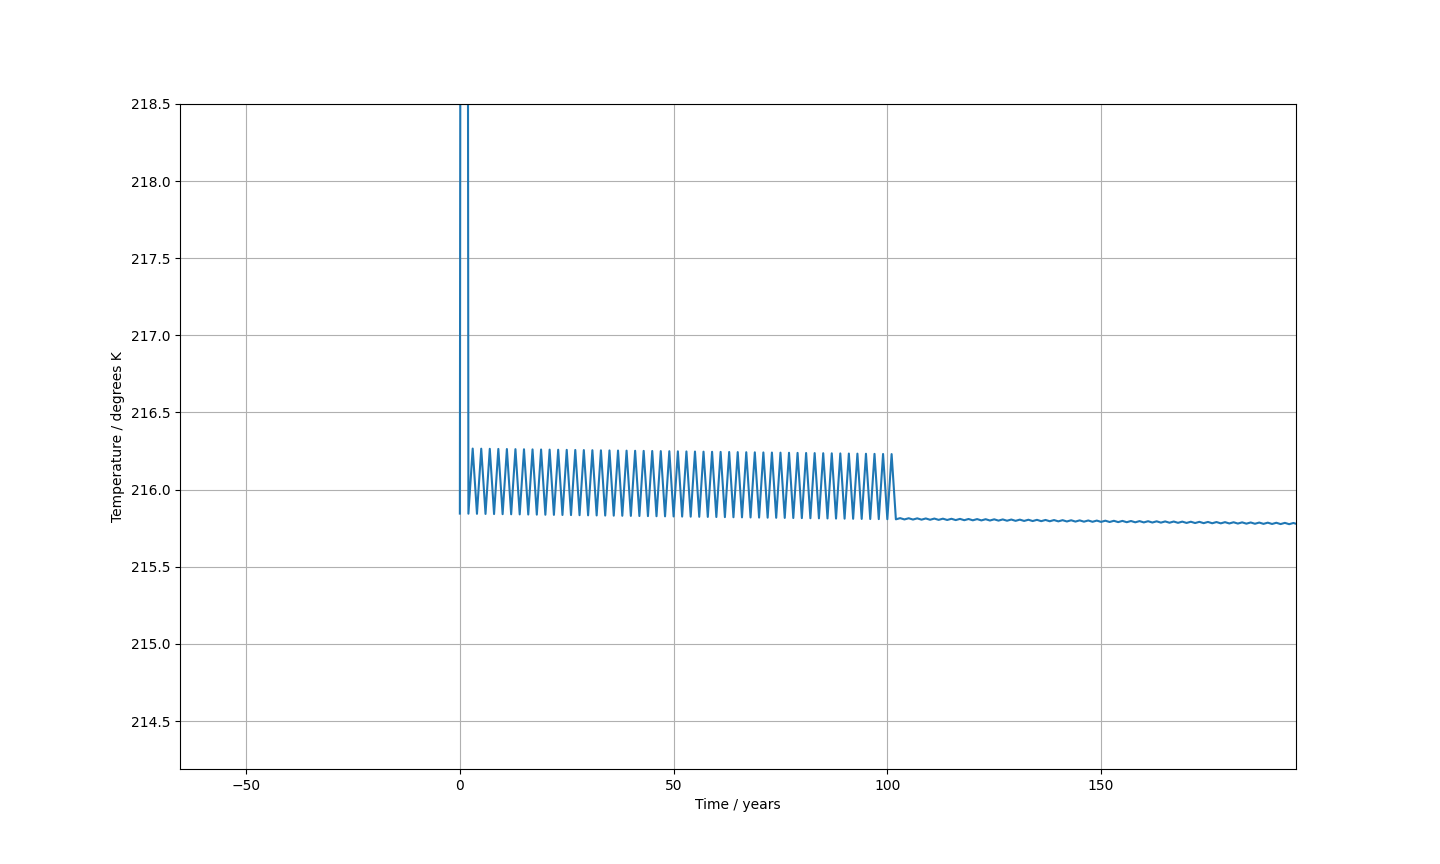
\includegraphics[scale=0.35]{Figure_3.png}
Figure 2 zoomed in
\end{center}

\subsection{Varying Parameters\label{varying-parameters}}

\begin{center}
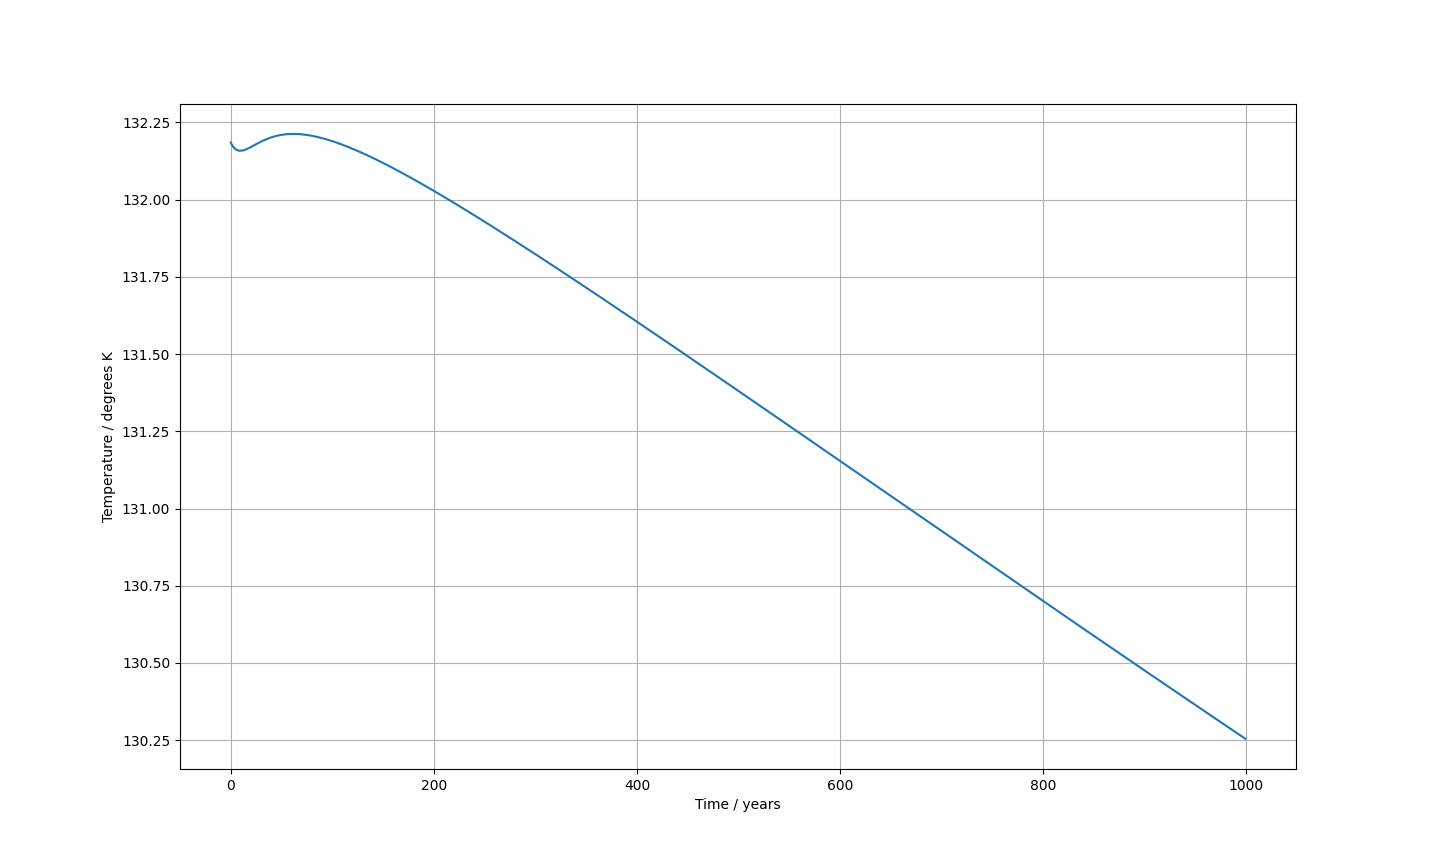
\includegraphics[scale=0.35]{Figure_4.png}
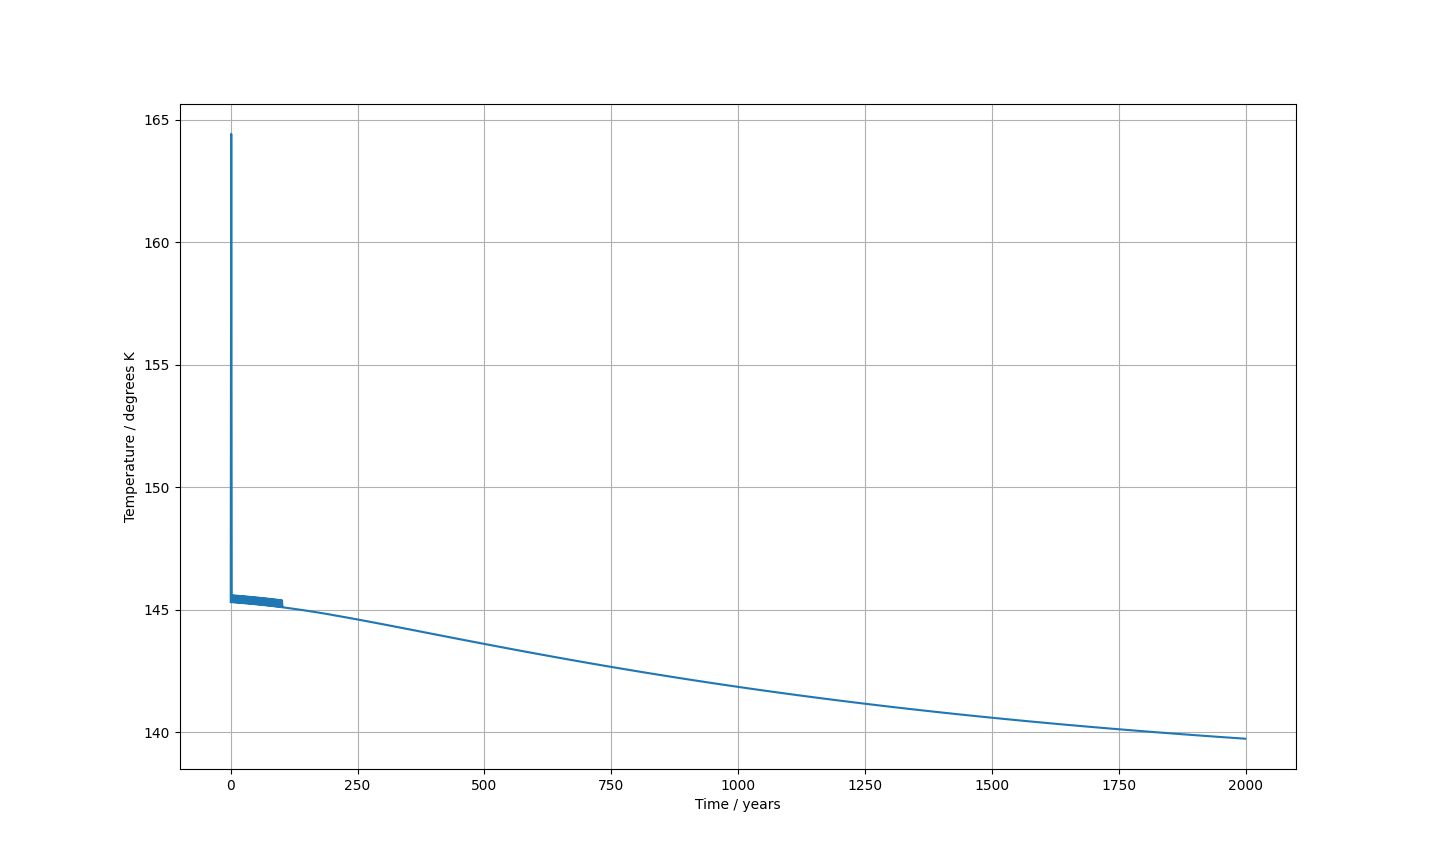
\includegraphics[scale=0.35]{Figure_5.png}
When the luminosity is doubled, but the distance is tripled, and the 
emissivity increases by 25\% the above results are produced
\end{center}

\begin{center}
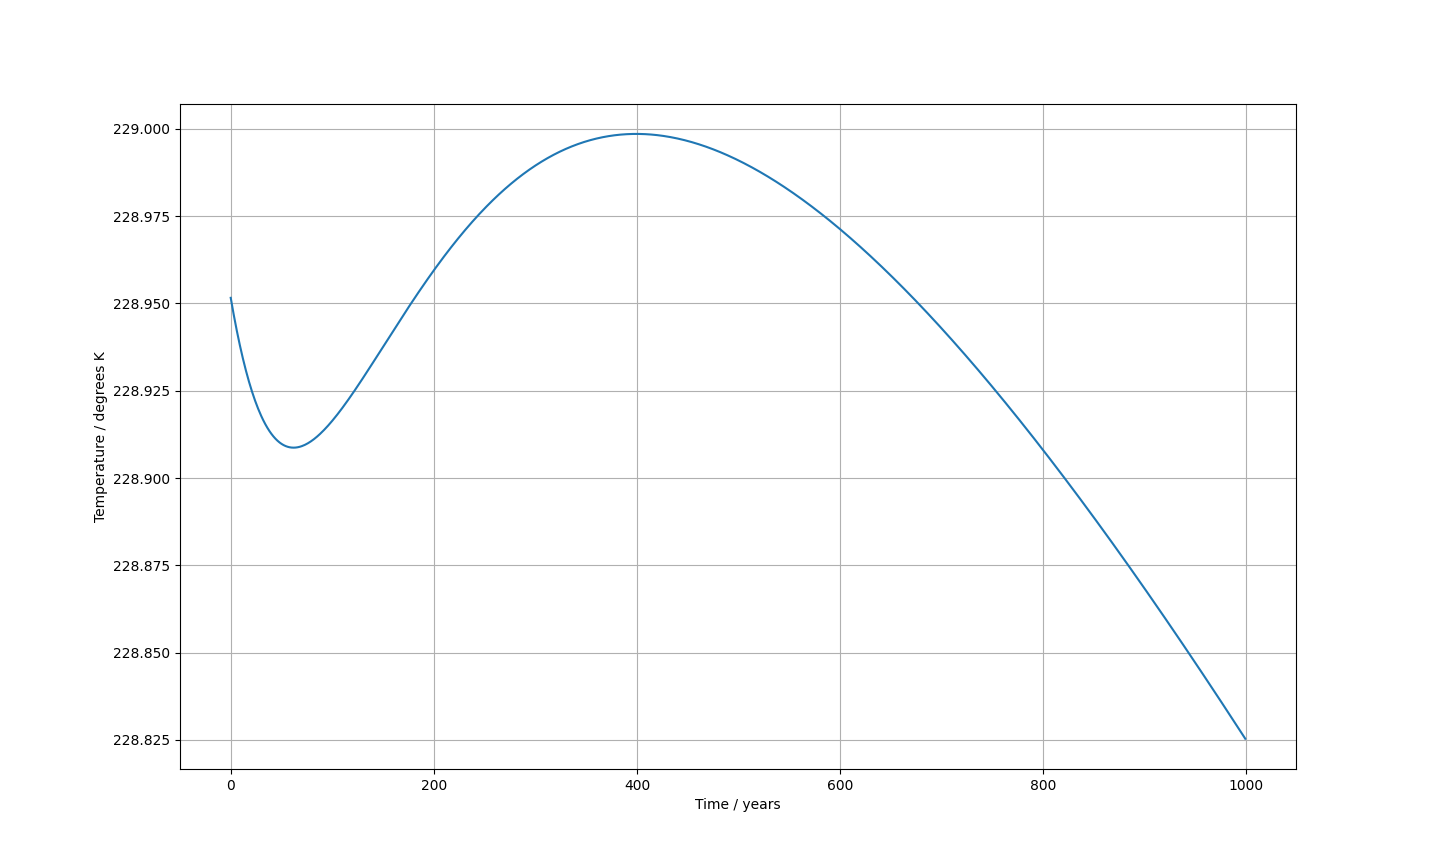
\includegraphics[scale=0.35]{Figure_6.png}
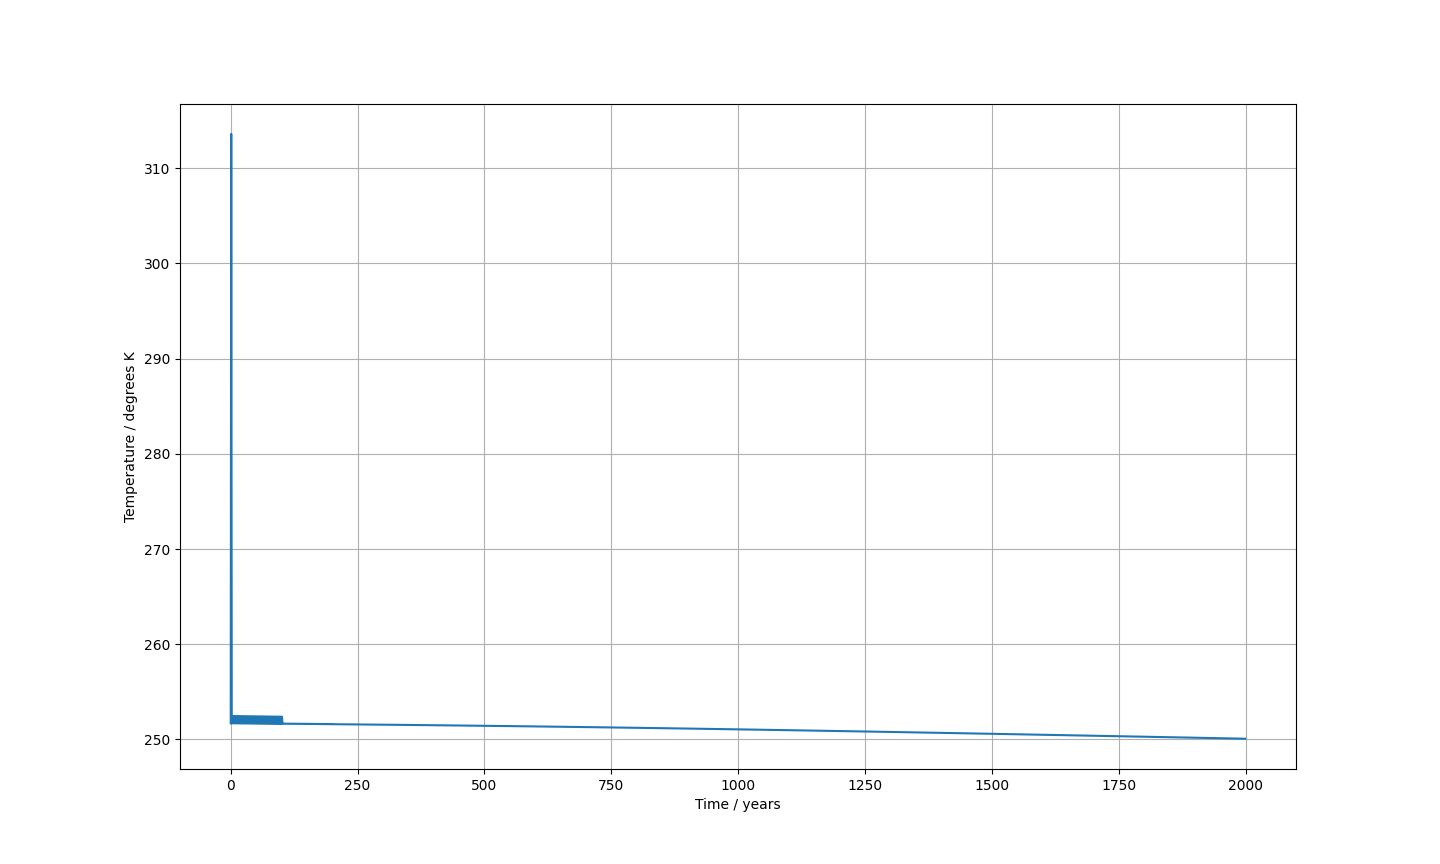
\includegraphics[scale=0.35]{Figure_7.png}
When the luminosity is doubled and the emissivity increases by 25\% the above results are produced
\end{center}

\newpage
\section{Conclusion and Final Thoughts}

\onehalfspacing{\noindent{In any case, the results this model produces are 
fairly accurate, but the trends, at least with the limited runtime are not 
looking promising. The average global temperature at the end of 1 run of the 
simulation is around 73\% accurate, however, I believe that the backbone and 
mathematics behind the model is all sound, and simply small errors in 
implementation or the assumptions which I took to avoid the model becoming 
too complex to handle have limited its success. Perhaps working with a 
partner would yield better results as 2 minds to deal with the complexity 
and implementation would have probably eliminated some minor errors and 
together, I and a partner could perhaps have come up with better ways to 
implement this project. \\}}

\onehalfspacing{\noindent{Given my limited knowledge of Python and best 
practices, there were probably better ways of implementation but I think 
that this model performs satisfactorily to well in that 75\% accuracy is 
pretty high given how many assumptions and simplifications I made. I would 
hope that the model produces better results when run for longer, but there 
is always the possibility that the downward trend continues and the accuracy 
decreases. However, global temperatures have reached lows of 150 to 160 
Kelvin in prehistory, so perhaps comparing my results of an earth that is 
only 1000 years old to today's earth of 4.6 billion years creates an unfair 
margin. This project could be improved but given my limited knowledge of 
python, geography and physics, I believe that this was a good first attempt 
at modelling the climate, an undoubtedly very complex task. Given more time, 
I would like to further investigate the effects of time and also change 
certain parameters to get a better understanding of their effect on the 
climate.}}


\newpage
\section{Bibliography and Notes\label{bibliography-and-notes}}
\begin{thebibliography}{15}
\RaggedRight
\bibitem{1} https://www.usgs.gov/special-topics/water-science-school/science/how-much-water-there-earth 

https://education.seattlepi.com/percent-earth-permanently-covered-snow-ice-4666.html

\bibitem{2} This definition is taken and paraphrased from https://www.sciencedirect.com/topics/chemical-engineering/heat-flux

\bibitem{3} This equation is the differential form of Fourier’s law, according to https://en.wikipedia.org/wiki/Thermal\_conduction\#Fourier's\_law

\bibitem{4} https://en.wikipedia.org/wiki/Stefan–Boltzmann\_law

\bibitem{5} The full derivation of this equation can be found at https://en.wikipedia.org/wiki/Idealized\_greenhouse\_model

\bibitem{6} Contributions from the cryosphere and lithosphere are much lesser according to Enderton, 2009 and are therefore considered negligible in my model to decrease the complexity and make the model easier to deal with. https://core.ac.uk/download/pdf/4412312.pdf

\bibitem{7} “Ocean circulation is probably responsible for 30\% of the poleward transport of heat, leaving a contribution of 70\% for the atmosphere (Wunsch, 2005), quoted in Rummel, 2020

\bibitem{8} https://en.wikipedia.org/wiki/List\_of\_thermal\_conductivities

\bibitem{9} https://en.wikipedia.org/wiki/Antarctic\_ice\_sheet

\bibitem{10} https://climate.nasa.gov/vital-signs/ice-sheets

\bibitem{11} https://climate.nasa.gov/news/2948/milankovitch-orbital-cycles-and-their-role-in-earths-climate

\bibitem{12} https://www.climate.gov/news-features/climate-qa/hasnt-earth-warmed-and-cooled-naturally-throughout-history

\bibitem{13} https://www.nature.com/scitable/knowledge/library/milankovitch-cycles-paleoclimatic-change-and-hominin-evolution-68244581

\bibitem{14} https://climate.nasa.gov/news/2948/milankovitch-orbital-cycles-and-their-role-in-earths-climate/

\bibitem{15} https://www.obviously.ai/post/machine-learning-model-performance

\end{thebibliography}

\end{document}